\chapter{INTRODUCTION}
\label{ch:intro}
% \textbf{Motivation---why you should read this thesis
% What is this thesis about?}
% At first glance, the Universe appears to be an overwhelmingly vast and complicated place.
% However upon closer inspection, it is comprised of only a few different kinds of fundamental particles.
% Particle physics has given rise to the Standard Model (SM) which mathematically describes these constituents and their interactions with each other.
The Universe, while overwhelmingly vast, is built from a remarkably few kinds of elementary
% comprised of curiously few
% ---\emph{indivisible}---particles.
(\ie indivisible) particles.
% a curiously small number of elementary particle types.
As shown in Fig.~\ref{fig:particular_table}, any elementary particle can be classified into 1 of these 3 categories:
%%%%%%%%%%%%%%%%%%%%
\begin{figure}[!b]
    \centering
    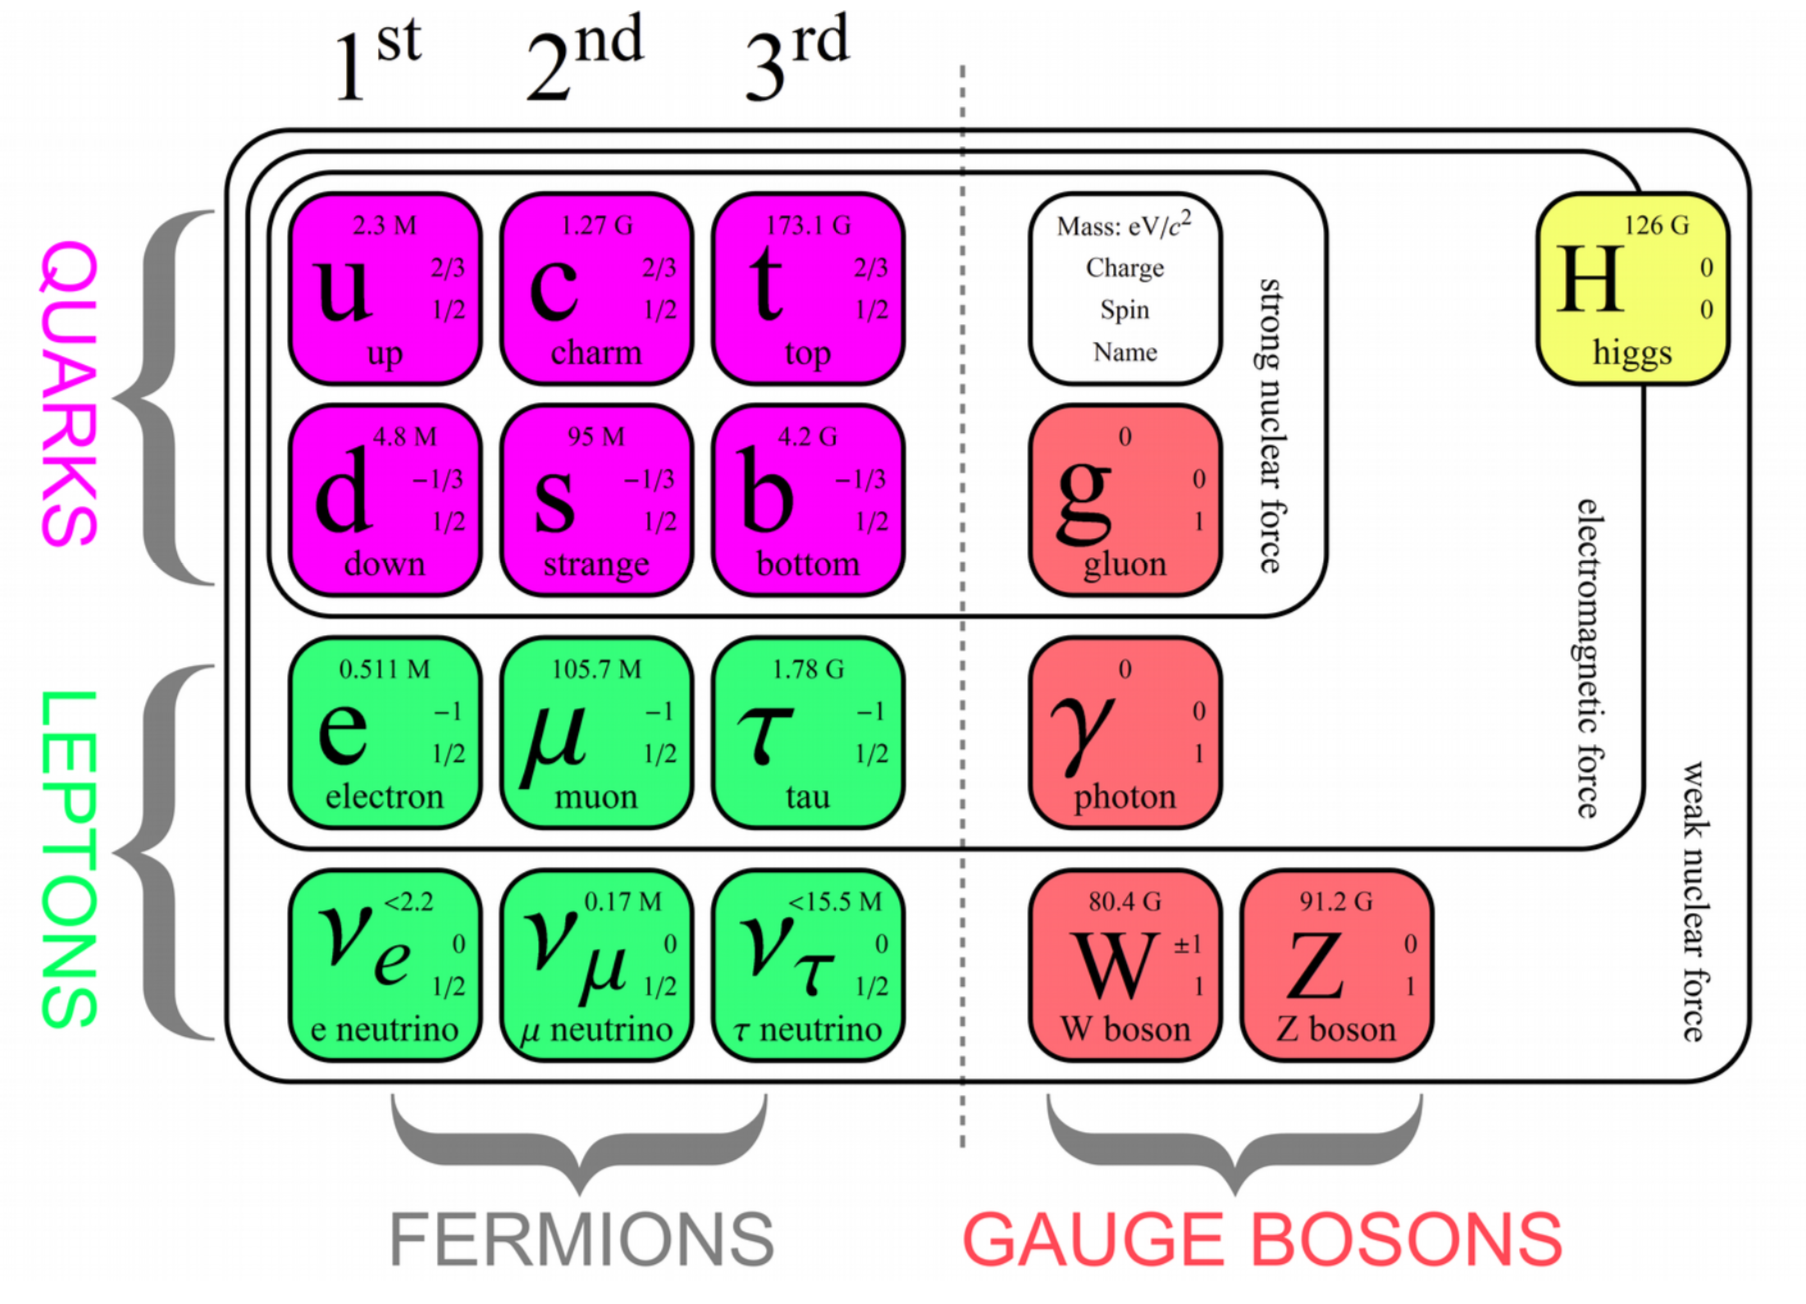
\includegraphics[height=9cm,keepaspectratio]{figures/sm/particular_table_updated.png}
        \caption
            [The elementary particles described by the SM]
            {The elementary particles described by the SM.}
        \label{fig:particular_table}
\end{figure}
%%%%%%%%%%%%%%%%%%%%
matter particles (\emph{fermions}), force-carrying particles (\emph{gauge bosons}), and Higgs bosons.
% ---the only scalar particle so far discovered.
% There are 12 kinds of matter particles (\emph{fermions}), the 4 kinds of force-carrying particles (\emph{gauge bosons}), and the singular kind of Higgs boson---the only scalar particle so far discovered.
% ---of which there are 6 kinds of quarks and 6 kinds of leptons---and the force-carrying particles (gauge \emph{bosons})---of which there are 4 kinds.
There are 12 kinds of fermions which can be split evenly into 2 groups, depending on with which forces they interact:
those that interact via the electromagnetic (EM) force and the weak nuclear force are classified as \emph{leptons}, of which there are 6 kinds (\emph{``flavors''}),
whereas those that interact via the EM, weak, \emph{and} strong nuclear forces are classified as \emph{quarks}, of which there are also 6 flavors.
There are 4 kinds of gauge bosons, each of which is a force carrier for a specific force
(the gluon is said to \emph{mediate} the strong force, the photon mediates the EM force, while the \PWpm and \PZ bosons mediate the weak force).
% Depending on through which forces the particles interact,  split into 6 kinds of \emph{quarks} (strong, weak, and electromagnetic) and 6 kinds of \emph{leptons} (weak and electromagnetic).
% Fermions can be split further into 6 kinds of quarks and 6 kinds of leptons,
% while the 
% only 12 kinds of \emph{matter} particles (green and pink) that comprise all detectable matter,
% 4 \emph{force} particles (red) that convey forces between the matter particles.
Thus, all the diversity and manifestations of reality come from only 17 kinds of ``building blocks''.
% While it is fascinating to wonder how so much diversity can arise from just 17 ``simple'' building blocks, the mission of particle physicists is to understand the underlying mathematical structure that describes Nature in as concise---and accurate---a theory as possible.
It is the mission of particle physicists to understand the underlying mathematical structure that describes Nature in as accurate---and concise---a theory as possible.
The best theory that stands today is called the Standard Model (SM) of particle physics.

%(see Chapter~\ref{ch:theory} for a mathematical overview).
% Universe metastability.
% , the SM accurately describes most of the properties of the eleme
% Although the SM will be mathematically outlined in Chapter~\ref{ch:theory}, it is 
The SM has bore witness to many triumphs over its approximately 70-year development:
it predicted the existence of quarks which were experimentally confirmed in the mid-1970s;
it predicted the existence of the tau neutrino which was experimentally confirmed in 2000;
its most groundbreaking prediction was experimentally confirmed on July 4, 2012---just shy of 10 years ago from the date of this dissertation writing---when the ATLAS and CMS collaborations announced the discovery of the Higgs boson~\cite{chatrchyan_observation_2012, aad_observation_2012, chatrchyan_observation_2013}.

% THE HIGGS IS IMPORTANT BECAUSE it was the missing piece of the SM.
Quantum Field Theory is the mathematical and conceptual backbone of the SM.
Within its framework, all particles are \emph{excitations} of their corresponding field so, \eg \emph{every} electron in the Universe is thought to be an excitation of the one and only electron field that permeates all of spacetime.
The existence of the Higgs boson (\PH) suggests that its corresponding field exists---the \emph{Higgs field}---and, thus, \PH is the quantum excitation of that field.
This all-pervasive Higgs field and its associated boson are generated mathematically via the Brout--Englert--Higgs mechanism (Sec.~\ref{sec:higgs_mech}).
The charged fermions within the SM ``acquire'' their mass by interacting with the Higgs field.
This is also how the Higgs boson itself acquires its mass (\mH)---by interacting with its own field.

% The masses of SM particles \emph{depend} on the value of \mH\ldots \emph{so what is its value?}
Unfortunately, \mH is a free parameter of the SM, so theory is unable to provide a value for \mH based solely on other fundamental constants. % TODO: get mH formula and fix this line.
Thus, \mH must be experimentally measured.
Although \mH has already been measured~\cite{chatrchyan_observation_2012, aad_observation_2012, chatrchyan_observation_2013, PhysRevLett.114.191803, the_cms_collaboration_precise_2015, HIG_16_041, aaboud_measurement_2018, CMS-PAS-HIG-18-029, ATLAS-CONF-2019-025, sirunyan_measurement_2020}, it is important to continually improve the precision on the measurement by lowering the corresponding uncertainties on the mass value.
A more precise value of \mH is two-fold:
first, it improves the theoretical limits on the masses of the other elementary particles and, second, it very well may determine the stability of our universe, as shown in Fig.~\ref{fig:universe_stability}.
% it predicts that all particles---especially the electroweak bosons should be massless
% ,  Particles interact with it and acquire their mass---all except neutrinos and massless bosons.
% Since its conceptualization in 1964, the Higgs boson remained undetected for 48 years until its confirmed production at the LHC. 
%%%%%%%%%%%%%%%%%%%%
\begin{multiFigure}
    \centering
    \addFigure{0.48}{figures/intro/mtop_vs_mH_universestability_zoomout.png}
    \addFigure{0.48}{figures/intro/mtop_vs_mH_universestability_zoomin.png}
    \captionof{figure}
        [Theoretical stability regions of the Universe]
        {Theoretical stability regions of the Universe.
        A) Stability regions of the Universe based on the pole masses of the top quark $\left( \mass{t}^\text{pole} \right)$ and Higgs boson $\left( \mass{h}^\text{pole} \right)$.
        B) Closeup of the SM region in (A).
        The contours represent 68\%, 95\%, and 99\% confidence levels based on the experimental uncertainties of $\mass{t}^\text{pole}$ and $\mass{h}^\text{pole}$.
        Plots taken from~\cite{univ_stab} and units added to all axes.
        }
    \label{fig:universe_stability}
\end{multiFigure}
%%%%%%%%%%%%%%%%%%%%

The production of a Higgs boson is only feasible at conditions close to those thought to exist at the beginning of the Universe.
%   elusive Higgs boson (\PH) is ONLY MADE AT CRAZY CONDITIONS.
This grand achievement is accomplished frequently by the Large Hadron Collider (LHC), located on the border of France and Switzerland.
It is the largest and most powerful proton--proton (\pp) collider ever made.
The LHC accelerates protons to incredible speeds, very close to the speed of light.
When these fast-moving protons collide, the \pp collisions can have a center-of-mass energy as high as 13\TeV.
Newly produced particles spew out of the collision points and are analyzed by detectors like the aforementioned ATLAS and CMS experiments.
These enormous particle detectors have thousands of scientists performing dozens of analyses to look for hints of beyond Standard Model (BSM) physics, extra dimensions, miniature black holes, and more.

This dissertation summarizes the results from two different, but related, analyses.
The first analysis lays out the steps necessary in order to perform the world's best precision measurement of \mH to date, using data collected by the CMS experiment during the LHC Run 2 (2016--2018).
Although this dissertation was completed before the data could be unblinded and before the final measurement of \mH could be made,
expectations on the uncertainties of \mH are set and are predicted to reduce the world's current best precision from 14\MeV down to 11\MeV.
% presents the work done thus far in what is expected to be the world's most precise measurement of \mH.
The second analysis details the search for low-mass dilepton resonances in \htofourl decays and sets limits on related BSM branching fractions and on the Higgs-mixing parameter.
% This dissertation presents the world's most precise measurement of the Higgs boson mass (\mH) to date, using proton--proton collision data from the LHC Run 2, collected and analyzed by the CMS Experiment.

The following chapters of this dissertation begin by describing the function and engineering of the Large Hadron Collider in Chapter~\ref{ch:lhc}.
Then, a thorough description of the CMS experiment and its composite subdetectors is given in Chapter~\ref{ch:cms}.
Next, the first of two analyses---expectations for the precision measurement of the Higgs boson mass using the LHC Run 2 data---is detailed in Chapter~\ref{ch:higgs_mass}.
Afterwards, a the second of two analyses---a search for low-mass dilepton resonances in \htofourl decays---is outlined in Chapter~\ref{ch:dilep_res}.
Finally, the results of the expectations for the Higgs boson mass measurement is summarized in Chapter~\ref{ch:conclusion}.
% begins with a mathematical  the standard model (SM) of particle physics and its mathematical framework, including the Brout-Englert-Higgs (BEH) mechanism

% Chapter~\ref{ch:intro} (\emph{this chapter}) discusses the importance and motivation for measuring the mass of the Higgs boson;
% Chapter~\ref{ch:theory} introduces the standard model (SM) of particle physics and its mathematical framework, including the Brout-Englert-Higgs (BEH) mechanism;
% Chapter~\ref{ch:lhc};
% Chapter~\ref{ch:cms};
% Chapter~\ref{ch:higgs_mass};
% Chapter~\ref{ch:dilep_res};
% Finally, Chapter~\ref{ch:conclusion}.








% Many properties of these particles---and their interactions with each other---are accurately described by the standard model (SM) of particle physics.
% Problematically though, the SM predicts that the gauge bosons (the particles which convey forces) particles are massless.
% The most significant triumph of the SM occurred on July 4$^\text{th}$, 2012 when the ATLAS and CMS collaborations announced the discovery of the ``missing puzzle piece'' of the SM---the Higgs boson.

% This discovery confirmed the SM's prediction that there should exist, which date back to 1964 via the Brout-Englert-Higgs mechanism
% In the SM, particle interactions are conveyed by way of 3 fundamental forces, the strong, weak, and electromagnetic forces, while the 4th force---gravity---is neglected due to its negligible contribution at nuclear distances.
% The seed of the most successful triumph of the SM dates back to 1964, when physicists Robert Brout, François Englert, and Peter Higgs , which occurred on July 4th, 2012, was possible its most spectacular: the when the Higgs boson was  The prediction capabilities of the SM are 
% strong, weak, and electromagnetic interactions
% By understanding the rules by which these particles interact, we can ;
% this is the aim of the Standard Model (SM) of Particle Physics. 
% The Standard Model (SM) is an impressively accurate mathematical theory which describes the fundamental particles of the universe and the rules for their possible interactions.
% 
%  are described mathematically by the impressively accurate Standard Model (SM) of Particle Physics.
% Although there are four fundamental forces of nature, the SM takes into account three of the four forces in nature:
% The Higgs boson (\PH) was the so-called a critical piece of the SM because, without it,  it is the quantum excitation of the so-called Higgs field, an all-pervasive field throughout spacetime 

% It is necessary to scrutinize the properties of this new particle to check whether it truly is the \PH predicted by the SM---or perhaps something else entirely.

% A major shortcoming of the SM is its inability to predict the masses of these particles.

% The SM was not able to predict the masses of these particles until 1964 when the Brout-Englert-Higgs mechanism suggested that 
% It wasn't until 1964 that the Brout-Englert-Higgs mechanism gave a self-consistent way to :
% by breaking the electroweak gauge symmetry of the vacuum would give rise to non-zero masses of the weak gauge bosons.
% This would yield a secondary effect too:
% there should exist a fundamental scalar boson which is the quantum of the so-called ``Higgs field''.
% On July 4th, 2012, this Higgs boson was discovered.